\documentclass[12pt,
               a4paper, 
               english,          % Hifenizacoes em ingles
               brazil            % Ultimo idioma é o padrao do documento
               ]{report}

%Dados que precisam ser customizados em todo projeto. Ex.: Titulo, Autor, Orientador, etc 
\makeatletter
\newcommand{\cidade}[1]{\gdef\@cidade{#1}}
\newcommand{\faculdade}[1]{\gdef\@faculdade{#1}}
\newcommand{\faculdadesigla}[1]{\gdef\@faculdadesigla{#1}}
\newcommand{\instcomp}[1]{\gdef\@instcomp{#1}}
\newcommand{\instnce}[1]{\gdef\@instnce{#1}}
\newcommand{\instncecurto}[1]{\gdef\@instncecurto{#1}}
\newcommand{\programa}[1]{\gdef\@programa{#1}}
\newcommand{\progsigla}[1]{\gdef\@progsigla{#1}}
\newcommand{\orientadora}[1]{\gdef\@orientadora{#1}}
\newcommand{\coorientadora}[1]{\gdef\@coorientadora{#1}}
\newcommand{\orientadorastitulo}[1]{\gdef\@orientadorastitulo{#1}}
\newcommand{\textofolharosto}[1]{\gdef\@textofolharosto{#1}}


\title{Titulo Completo do Trabalho}
\author{Nome do(a) Autor(a) do Trabalho}
\date{2025}
\cidade{Rio de Janeiro}
\faculdade{Universidade Federal do Rio de Janeiro}
\faculdadesigla{UFRJ}
\instcomp{Instituto de Computação}
\instnce{Instituto Tércio Pacitti de Aplicações e Pesquisas Computacionais}
\instncecurto{Instituto Tércio Pacitti de Aplicações}
\programa{Programa de Pós-Graduação em Informática}
\progsigla{PPGI}
\orientadora{Nome do(a) Orientador(a)}
\coorientadora{Nome do(a) Co-orientador(a)}
\orientadorastitulo{D.SC}
\textofolharosto{Dissertação de Mestrado apresentada ao \@programa, \@instcomp\ e  \@instnce, \@faculdade, como requisito parcial à obtenção do título de Mestre em Informática.}
\makeatother

%Configurações gerais do projeto, normalmente não precisam ser alterados
\usepackage[brazilian]{babel}              % Traduções utilizados por vários pacotes
\usepackage[top=3cm,                    % definição padrao das margens das paginas
            bottom=2cm,
            left=3cm,
            right=2cm]{geometry}
\usepackage{opensans}                    % Pacote da fonte escolhida: Opções de fontes em: https://ctan.org/topic/font
\usepackage{lscape}                     % permite colocar um conteudo em formato paisagem (rotacionar)
\usepackage{color}                      % Permite utilizar cores pelos nomes
\usepackage{microtype}     			    % para melhorias de justificação
\usepackage[indentfirst=false]{quoting} % Usado para citação
\usepackage{url}                        % Usado para formatar URLs no texto
\usepackage{enumitem}                   % Permite alterar o formato das listas enumeradas 
\usepackage{booktabs}                   % Usado para personalizar elementos em tabelas, como \toprule e \midrule
\usepackage{arydshln}                   % Usado para personalizar elementos em tabelas, como \cdashline
\usepackage{amsmath}                    % Usado nas referencias de equações, através do comando \eqref
\usepackage{float}                      % Necessario para posicionar as figuras e tabelas de forma flutuante
\usepackage{svg}                        % Pacote que permite utilização de imagens SVGs (vetoriais) no documento 
\usepackage{pdfpages} % Necessario para incluir a ficha catalográfica


% Usando pacote de estilos de referencias bibliograficas (estilo IBICT complero)
\usepackage[style=3-pos-textuais/instituto-brasileiro-de-informacao-em-ciencia-e-tecnologia-abnt]{citation-style-language}
\addbibresource{3-pos-textuais/referencias_bibliograficas.bib}



%%%%% Redefinindo localização da paginação - INICIO %%%%%%%%%%%%%%%%%%%%%%%%
\setlength{\headheight}{15pt} %Corrige warning do header do pacote fancyhdr
\usepackage{fancyhdr} % Pacote utilizado para alterar a posicao da paginação
\pagestyle{fancy}
\fancyhf{} % Limpa todos os cabeçalhos e rodapés padrão
\fancyhead[R]{\thepage} % Coloca o número da página no canto superior direito
\renewcommand{\headrulewidth}{0pt} % Remove a linha do cabeçalho (opcional)
\fancypagestyle{plain}{
    \fancyhf{} % Limpa cabeçalhos e rodapés
    \fancyhead[R]{\thepage} % Número da página no canto superior direito
    \renewcommand{\headrulewidth}{0pt} % Remove a linha do cabeçalho
}
%%%%%% Redefinindo localização da paginação - FIM %%%%%%%%%%%%%%%%%%%%%%%%



%%%%% Removendo da contagem as a capa e a ficha catalográfica - INICIO  %%%%%%%%%%%%%%%%%%%%%%%%
\addtocounter{page}{-2} 
%%%%% Removendo da contagem as a capa e a ficha catalográfica - FIM  %%%%%%%%%%%%%%%%%%%%%%%%



%%%%% Configuração do espacamento padrão do documento - INICIO  %%%%%%%%%%%%%%%%%%%%%%%%
\usepackage{setspace}  % pacote usado para define o espacamento entre linhas do texto e de partes especificas
\onehalfspacing % definindo espaçamento padrao de 1,5 nas entrelinhas
%%%%% Configuração do espacamento padrão do documento - FIM  %%%%%%%%%%%%%%%%%%%%%%%%



%%%%% Configurações de links das referencias internas e externos - INICIO  %%%%%%%%%%%%%%%%%%%%%%%%
\usepackage{hyperref} % Cria os links das referencias internas e para links externos tb
\makeatletter
\hypersetup{
    pdftitle={\@title},
    pdfpagemode=FullScreen,
    colorlinks=true,      % Ativa a coloração dos links
    linkcolor=black,     % Cor dos links internos
    citecolor=black,     % Cor das citações
    urlcolor=black       % Cor dos links de URL
}
\makeatother
%%%%% Configurações de links das referencias internas e externos - FIM  %%%%%%%%%%%%%%%%%%%%%%%%



%%%%% Configurações do texto de Fonte das imagens - INICIO  %%%%%%%%%%%%%%%%%%%%%%%%
\usepackage{copyrightbox} % Necessario para adicionar origem das imagem e das tabelas
\makeatletter
\renewcommand{\CRB@setcopyrightfont}{%
\color{black}
}
\makeatother
%%%%% Configurações do texto de Fonte das imagens - FIM  %%%%%%%%%%%%%%%%%%%%%%%%



%%%%% Evita reiniciar numeracoes das equações nos capitulos - INICIO  %%%%%%%%%%%%%%%%%%%%%%%%
\usepackage{chngcntr} % Permite modificar a numeração dos contadores: Equacoes, Tabelas, e Figuras
\counterwithout{equation}{chapter} % Remove a reinicialização da numeração a cada capítulo
% A configuração de tabela e figura estão em  seus respectivos arquivos de listagem 
% juntamente com as suas demais configurações 
%%%%% Evita reiniciar numeracoes das equações nos capitulos - FIM  %%%%%%%%%%%%%%%%%%%%%%%%

%%%%% Formatação da lista de figura e de tabelas - INICIO  %%%%%%%%%%%%%%%%%%%%%%%%
\usepackage{titletoc} % Pacote para formatar sumário, lista de figuras e tabelas

%a configuração só funciona se for antes do documentclass

%Lista de Tabelas
\titlecontents{figure}[0pt]
{}
{\figurename\ \thecontentslabel\ - }
{}
{\titlerule*[0.4pc]{.}\contentspage}
[\addvspace{5pt}]

%Lista de Tabelas
\titlecontents{table}[0pt]
{}
{\tablename\ \thecontentslabel\ - }
{ }
{\titlerule*[0.4pc]{.}\contentspage}
[\addvspace{5pt}]
%%%%% Formatação da lista de figura e de tabelas - FIM  %%%%%%%%%%%%%%%%%%%%%%%%



%%%%% Formatação dos titulos dos capitulos, secao, subsecao, etc - INICIO  %%%%%%%%%%%%%%%%%%%%%%%%
\usepackage{titlesec}

\titlespacing{\chapter}
  {0pt}   % Espaço à esquerda
  {-17pt}   % Espaço acima do título do capítulo (é aqui que se reduz)
  {15pt}  % Espaço abaixo do título do capítulo

\titleformat{\chapter}[hang] % shape
{\normalsize\bfseries\uppercase} % format
{\thechapter}
{10pt}
{}

\titleformat{\section}[hang] % shape
{\normalsize\normalfont\uppercase} % format
{\thesection}
{10pt}
{}

\titleformat{\subsection}[hang] % shape
{\normalsize\bfseries} % format
{\thesubsection}
{10pt}
{}

\titleformat{\subsubsection}[hang] % shape
{\normalfont\normalsize} % format
{\thesubsubsection}
{10pt}
{}

\titleformat{\paragraph}[hang] % shape
{\normalfont\normalsize} % format
{\theparagraph}
{10pt}
{}

\titleformat{\subparagraph}[hang] % shape
{\normalfont\normalsize} % format
{\thesubparagraph}
{}
{}
%%%%% Formatação dos titulos dos capitulos, secao, subsecao, etc - FIM  %%%%%%%%%%%%%%%%%%%%%%%%

% pacote que gera textos aletorios, pode remover quando for realizar o trabalho
\usepackage{lipsum} 


%%%%% Definindo diretorios padrao do template e do projeto - INICIO %%%%%%%%%%%%%%%%%%%%%%%%
\usepackage{graphicx}		            % Inclusão de gráficos, pdfs
\graphicspath{{figuras/}{figuras/template}}
%%%%% Definindo diretorios padrao do template e do projeto - INICIO %%%%%%%%%%%%%%%%%%%%%%%%

\begin{document}

%Includes pré-textuais
\thispagestyle{empty}
\newgeometry{top=4cm,bottom=1cm,left=3cm,right=3cm}
\makeatletter
\begin{center}


\includegraphics[width=1\textwidth]{logo_capa.pdf}

% As variáveis @author, @title, @subtitulo, @cidade e @date dessa página,
% podem ser ajustadas no arquivo config/informacoes_gerais.tex
\vspace{3cm}
\Large \@author

\vspace{2cm}
\Large \textbf{\MakeUppercase{\@title}\@subtitulo}

\vspace*{\fill}
\@cidade\\
\@date

\end{center}
\makeatother
\restoregeometry
\newpage

\thispagestyle{empty}
\makeatletter
\begin{spacing}{1}
\begin{center}

\large \MakeUppercase{\@faculdade}

\large \MakeUppercase{\@instcomp}

\large \MakeUppercase{\@instnce}

\large \MakeUppercase{\@programa} (\@progsigla)

\vspace{2cm}
\large \MakeUppercase{\@author}

\vspace{2cm}
\large \textbf{\MakeUppercase{\@title}\@subtitulo}
\end{center}

\vspace{0.5cm}
\epigraph{\normalsize\justifying\nohyphens{\@textofolharosto}}

\vspace{2cm}
Orientadora: Profa. \@orientadora, \@orientadorastitulo

Co-orientadora: Profa. \@coorientadora, \@orientadorastitulo

\vspace*{\fill}
\begin{center}
\@cidade\\
\@date
\end{center}

\end{spacing}
\makeatother
\newpage

\input{1-pre-textuais/ficha_catalografica}

\thispagestyle{empty}
\makeatletter
\begin{spacing}{1}
\begin{center}

\large \MakeUppercase{\@author}

\vspace{1.5cm}
\large \textbf{\MakeUppercase{\@title}\@subtitulo}

\end{center}

\vspace{0.5cm}
\epigraph{\normalsize\justifying\nohyphens{\@textofolharosto}}

\vspace{1.5cm}
Aprovado em 30 de março de 2025 por:

\vspace{2cm}
\begin{flushright}

\hspace{5cm} \hrulefill

Prof(a). \@orientadora, \@orientadorastitulo, \@progsigla/\@faculdadesigla (Presidente)

\vspace{2cm}
\hspace{5cm} \hrulefill

Prof(a). \@coorientadora, \@orientadorastitulo, \@progsigla/\@faculdadesigla

\vspace{2cm}
\hspace{5cm} \hrulefill

Prof(a). Nome do Representante da Banca, \@orientadorastitulo, NCE/\@faculdadesigla


\vspace{2cm}
\hspace{5cm} \hrulefill

Prof(a). Nome do Representante da Banca, \@orientadorastitulo, \@progsigla/\@faculdadesigla

\end{flushright}

\end{spacing}
\makeatother
\newpage

\thispagestyle{empty}
\begin{spacing}{1}
\vspace*{\fill}

\epigraph{\normalsize Dedico esse trabalho ao meus pais, por todo amor, dedicação e compreensão. Amo vocês.}

\end{spacing}
\newpage


\input{1-pre-textuais/agradecimentos}

\thispagestyle{empty}
\begin{spacing}{1}
\vspace*{\fill}

\epigraph{\normalsize\itshape``Descrever o texto da citacao utilizada na epígrafe desse template de trabalho.\\
O texto pode ter mais de uma linha caso se deseje.\\
Ou pode ser em um texto longo também. de acordo com a nacessidade e com a escolha feita.''}{(Nome do Autor)}

\end{spacing}
\newpage






\thispagestyle{empty}
\begin{center}
\textbf{\MakeUppercase{Resumo}}
\end{center}

\begin{spacing}{1.5}
Utilize, de preferência, um só parágrafo para descrever os objetivos de seu trabalho acadêmico, o método com informações sobre coleta, tratamento e análise dos dados, as técnicas de abordagem, os resultados e suas principais conclusões. Esse resumo deve conter de 150 a 500 palavras. Deve ser evitado o uso de frases negativas, símbolos ou contrações que não sejam de uso corrente, fórmulas, equações, diagramas etc. que não sejam absolutamente
necessários; quando for indispensável, defini-los na primeira vez que aparecerem. Texto adaptado do Manual do Sibi da UFRJ diponível em \cite{ManualSibi2023}.
\end{spacing}

\vspace{1em}

Palavras-chave: palavras; chaves; separadas; por; ponto e vírgula
\newpage

\thispagestyle{empty}
\begin{center}
\textbf{\MakeUppercase{Abstract}}
\end{center}

\begin{spacing}{1.5}
Traduza seu resumo para o idioma de
divulgação internacional escolhido por você e seu orientador. Traduza também as palavras-chave.
\end{spacing}

\vspace{1em}

Keywords: key; words; separated; by; semi commas
\newpage

\input{1-pre-textuais/lista_figuras}

\input{1-pre-textuais/lista_tabelas}

\input{1-pre-textuais/lista_siglas}

\addtocontents{toc}{\protect\thispagestyle{empty}} % força o "empty" na primeira pagina do sumário
\pagestyle{empty} % remove a nunemracao das demais paginas de sumario (se houver mais de uma) 

%apresenta ate o nivel 5, de paragrafo
\setcounter{tocdepth}{4}

%apresenta a numeracao ate o nivel 5, de paragrafo
\setcounter{secnumdepth}{4}

% titletoc - Configuração da formatação dos títulos (em seus vários níveis) no sumário. 
% A formatação desses mesmos títulos dentro do texto, precisa ser feito antes do begin{document} e ficou no arquivo: config/configuracoes.tex
\titlecontents{chapter}[12pt]
  {\normalfont\normalsize\bfseries}
  {\contentslabel{12pt}\uppercase} % removido \MakeUppercase
  {}
  {\titlerule*[0.4pc]{.}\contentspage} % aqui sim!

\titlecontents{section}[20pt]
  {\normalfont\normalsize}
  {\contentslabel{20pt}\uppercase}
  {}
  {\titlerule*[0.4pc]{.}\contentspage}

\titlecontents{subsection}[32pt]
  {\normalfont\normalsize\bfseries}
  {\contentslabel{32pt}}
  {}
  {\titlerule*[0.4pc]{.}\contentspage}

\titlecontents{subsubsection}[38pt]
  {\normalfont\normalsize}
  {\contentslabel{38pt}}
  {}
  {\titlerule*[0.4pc]{.}\contentspage}

\titlecontents{paragraph}[46pt]
  {\normalfont\normalsize}
  {\contentslabel{46pt}}
  {}
  {\titlerule*[0.4pc]{.}\contentspage}


%Altera e Formata o titulo do sumario
\renewcommand{\contentsname}{\normalsize\centerline{\bfseries\uppercase{Sumário}}}

\tableofcontents % Insere o sumário
\clearpage % Garante que o sumário termine aqui
\pagestyle{fancy} % Retorna ao estilo "fancy" para o restante do documents

%Includes p do texto principal
\chapter{Introdução}

Como exposto em \cite{Torralba2008}, o aprendizado de máquina tem sido utilizado como alternativa à implementação de algoritmos específicos e complexos durante a resolução de diversos tipos de problemas. 

\lipsum[6]

A Figura \ref{fig:mlapplications}, apresenta um breve resumo das possíveis aplicações do aprendizado de máquina.

\begin{figure}[ht]
    \centering
    \caption{Domínio de aplicações do aprendizado de máquina.}
    \copyrightbox[b]
    		{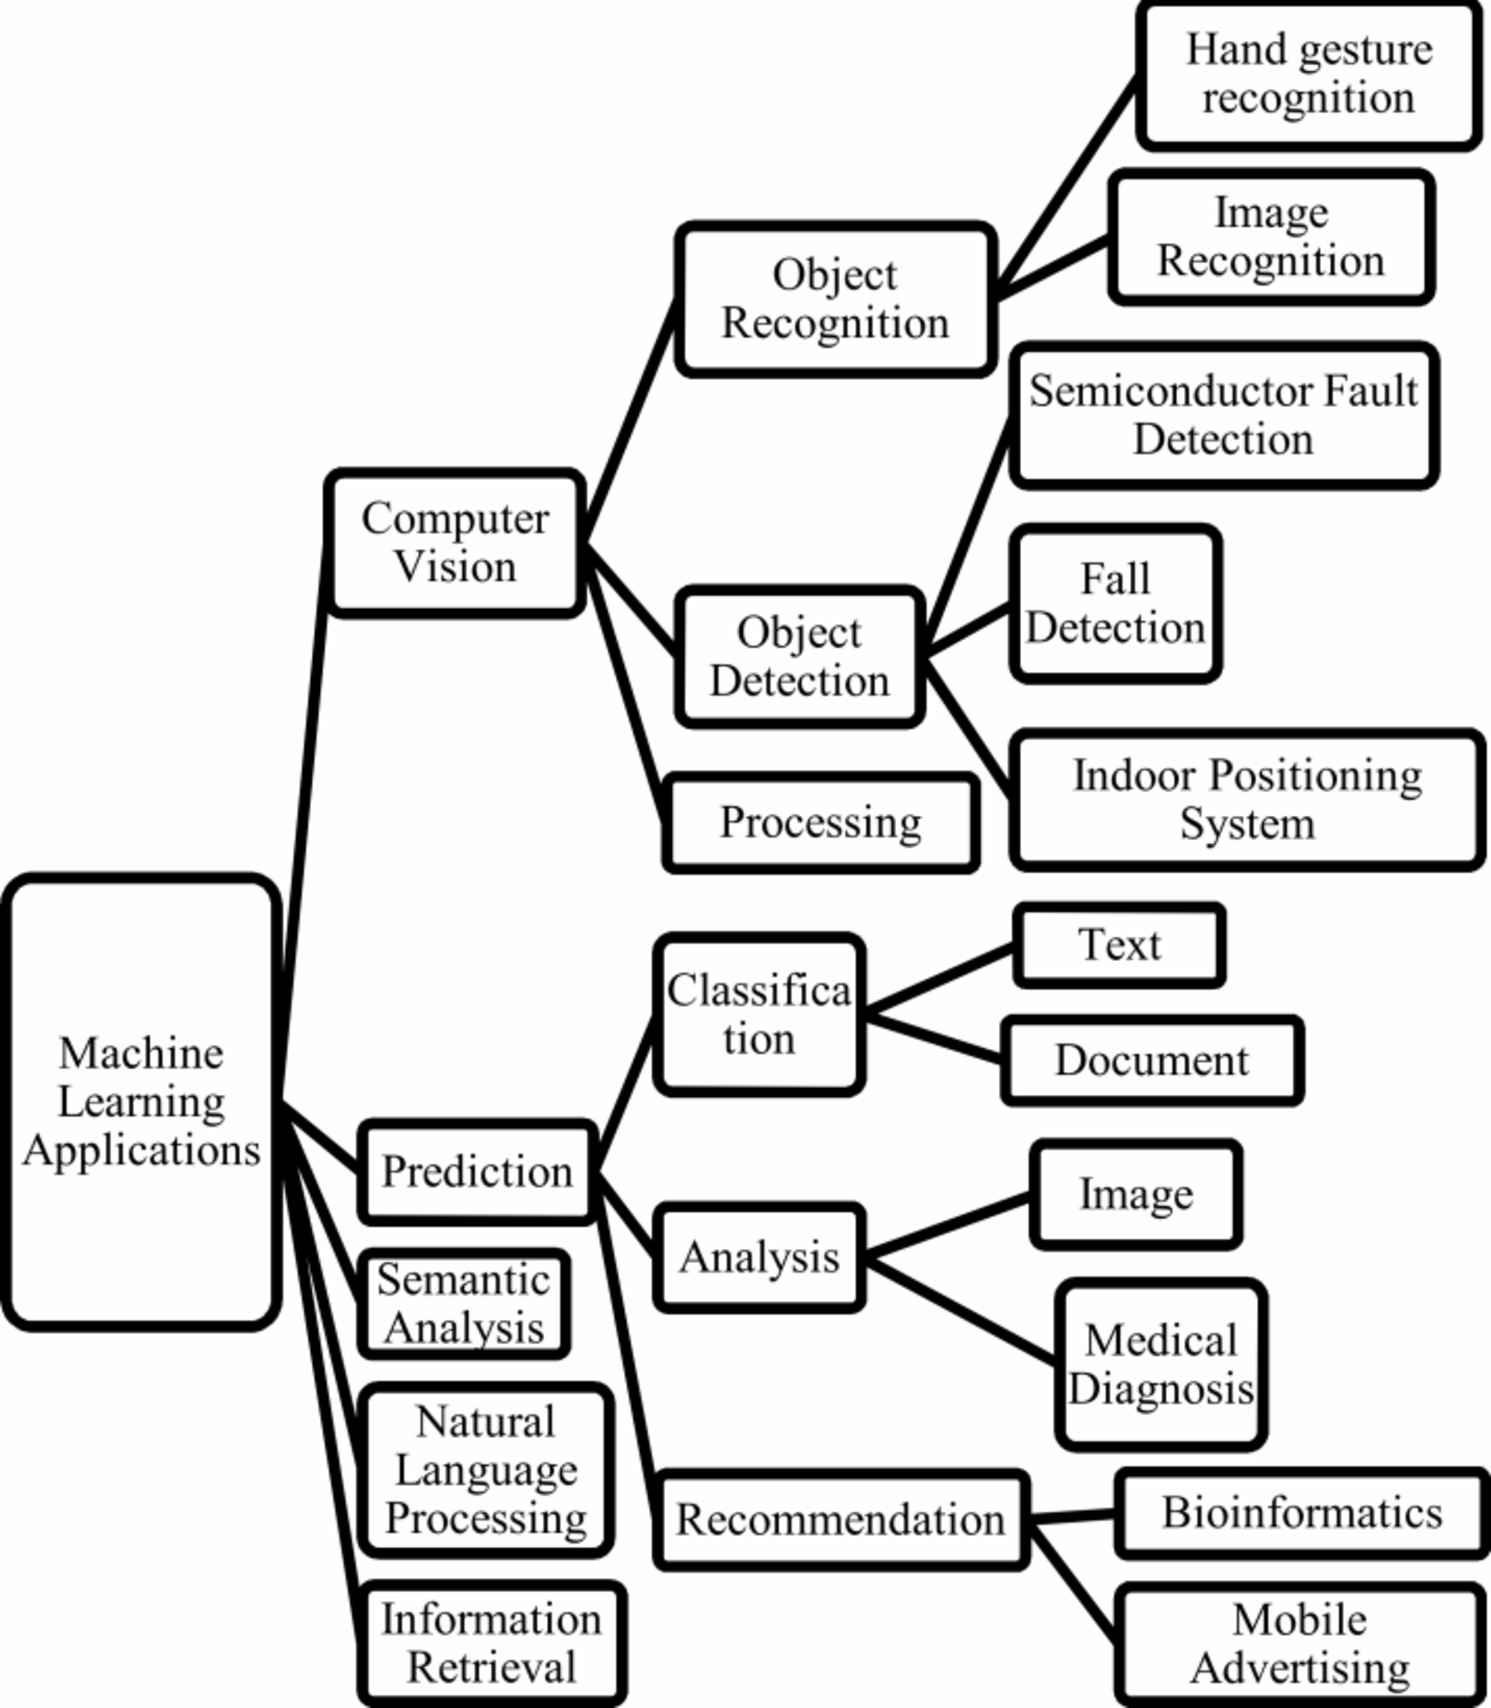
\includegraphics[width=0.7\linewidth]{mlapplications}}
            {Fonte: Extraída de \cite{ApplicationMachineLearning}}
    \label{fig:mlapplications}
\end{figure}

\lipsum[7-8]

\section{Motivação}

Como apresentado em \cite{mohri2018foundations}, com o resultado do desenvolvimento das tecnologias web, das redes sociais e dispositivos móveis, ocorreu uma verdadeira ``explosão'' no crescimento dos dados. 

\lipsum[9-16]


\section{Categorização do problema}

\lipsum[17-18]

\section{Proposta do trabalho}

\lipsum[19-21]

\section{Estrutura dessa trabalho}

O restante deste texto está organizado da seguinte forma. A Seção~\ref{cap:trabalhos_relacionados} contextualiza outros trabalhos que realizaram trabalhos similares. A Seção~\ref{cap:referencial_teorico} apresenta os conceitos básicos do referencial teórico necessário para um melhor entendimento do trabalho, com a apresentação dos assuntos tal, tal e tal. A Seção~\ref{cap:proposta_de_pesquisa} lista as questões da pesquisa, bem como seu objetivo principal e concluindo com as contribuições esperadas com o resultado final do trabalho. A Seção~\ref{cap:metodologia} demonstra qual foi a metodologia do trabalho. A Seção~\ref{cap:experimentos} explica como os experimentos foram executados. A Seção~\ref{cap:resultados} apresenta os resultados dos experimentos, Pot fim a Seção~\ref{cap:conclusao} apresenta um sumário dos resultados e sugestões para trabalhos futuros.

\input{2-textos/trabalhos_relacionados}

\chapter{Referencial teórico}
\label{cap:referencial_teorico}

Essa seção apresenta um pequeno conjunto de assuntos considerados pré-requisitos para um melhor entendimento desse trabalho.

\lipsum[22]

\section{Assunto 1 do referencial teórico} \label{sub:assunto2}

\lipsum[23-27]

\section{Assunto 2 do referencial teórico}

\lipsum[23-27]

\begin{enumerate}
    \item Exemplo de litstagem enumerada;
    \item Outro exemplo de de litstagem enumerada;
    \item Último exemplo de listagem enumerada.
\end{enumerate}

\lipsum[28]:

\begin{itemize}
    \item Exemplo de listagem com bullets;
    \item Outro exemplo de listagem com bullets; 
    \item Exemplo final de listagem com bullets. 
\end{itemize}

\section{Trabalhos relacionados}

\lipsum[23-27]

\chapter{Proposta de pesquisa}\label{cap:proposta_de_pesquisa}

Essa seção apresenta tanto as questões de pesquisa que norteiam a necessidade da mesma, bem como os objetivos primário e específicos relacionados ao trabalho.

\section{Questões de pesquisa} \label{sub:questpesq}

As perguntas que devem %pretendem 
ser respondidas ao final deste trabalho são apresentadas a seguir:

\begin{enumerate}[leftmargin=*, label=QP\arabic*:]
    \item Qual a primeira pergunta de pesquisa do trabalho?
    %\item É possível paralelizar o método FSP utilizando a linguagem Python?
    \item Qual seria outra pergunta de pesquisa do trabalho?
    \item Ainda tem mais pergunta de pesquisa para colocar aqui?
\end{enumerate}

\section{Objetivo principal}

O principal objetivo deste trabalho de pesquisa é "Descrever qual o principal objetivo deste trabalho de pesquisa".


\section{Contribuições esperadas}
As principais contribuições esperadas como resultado deste trabalho são:

\begin{enumerate}[leftmargin=*, label=CE\arabic*:]
    \item Primeira contribuição espera do trabalho;
    \item Segunda contribuição esperada do trabalho;
    \item Colocar quantas contribuições quiser.
\end{enumerate}

\chapter{Metodologia}\label{cap:metodologia}

Essa seção apresenta a metodologia a ser adotada no trabalho. Esse trabalho utilizou o modelo de trabalho acadêmico mantido no Projeto Jacurutu \cite{Projeto_Jacurutu}\footnote{A última versão do modelo para trabalhos acadêmicos do Projeto Jacuruto pode ser acessada em: \url{https://doi.org/10.5281/zenodo.16969842}}.


\lipsum[37-38]

\begin{figure}[ht]
    \centering
    \caption{Processo iterativo usado no desenvolvimento}
    \copyrightbox[b]
  		{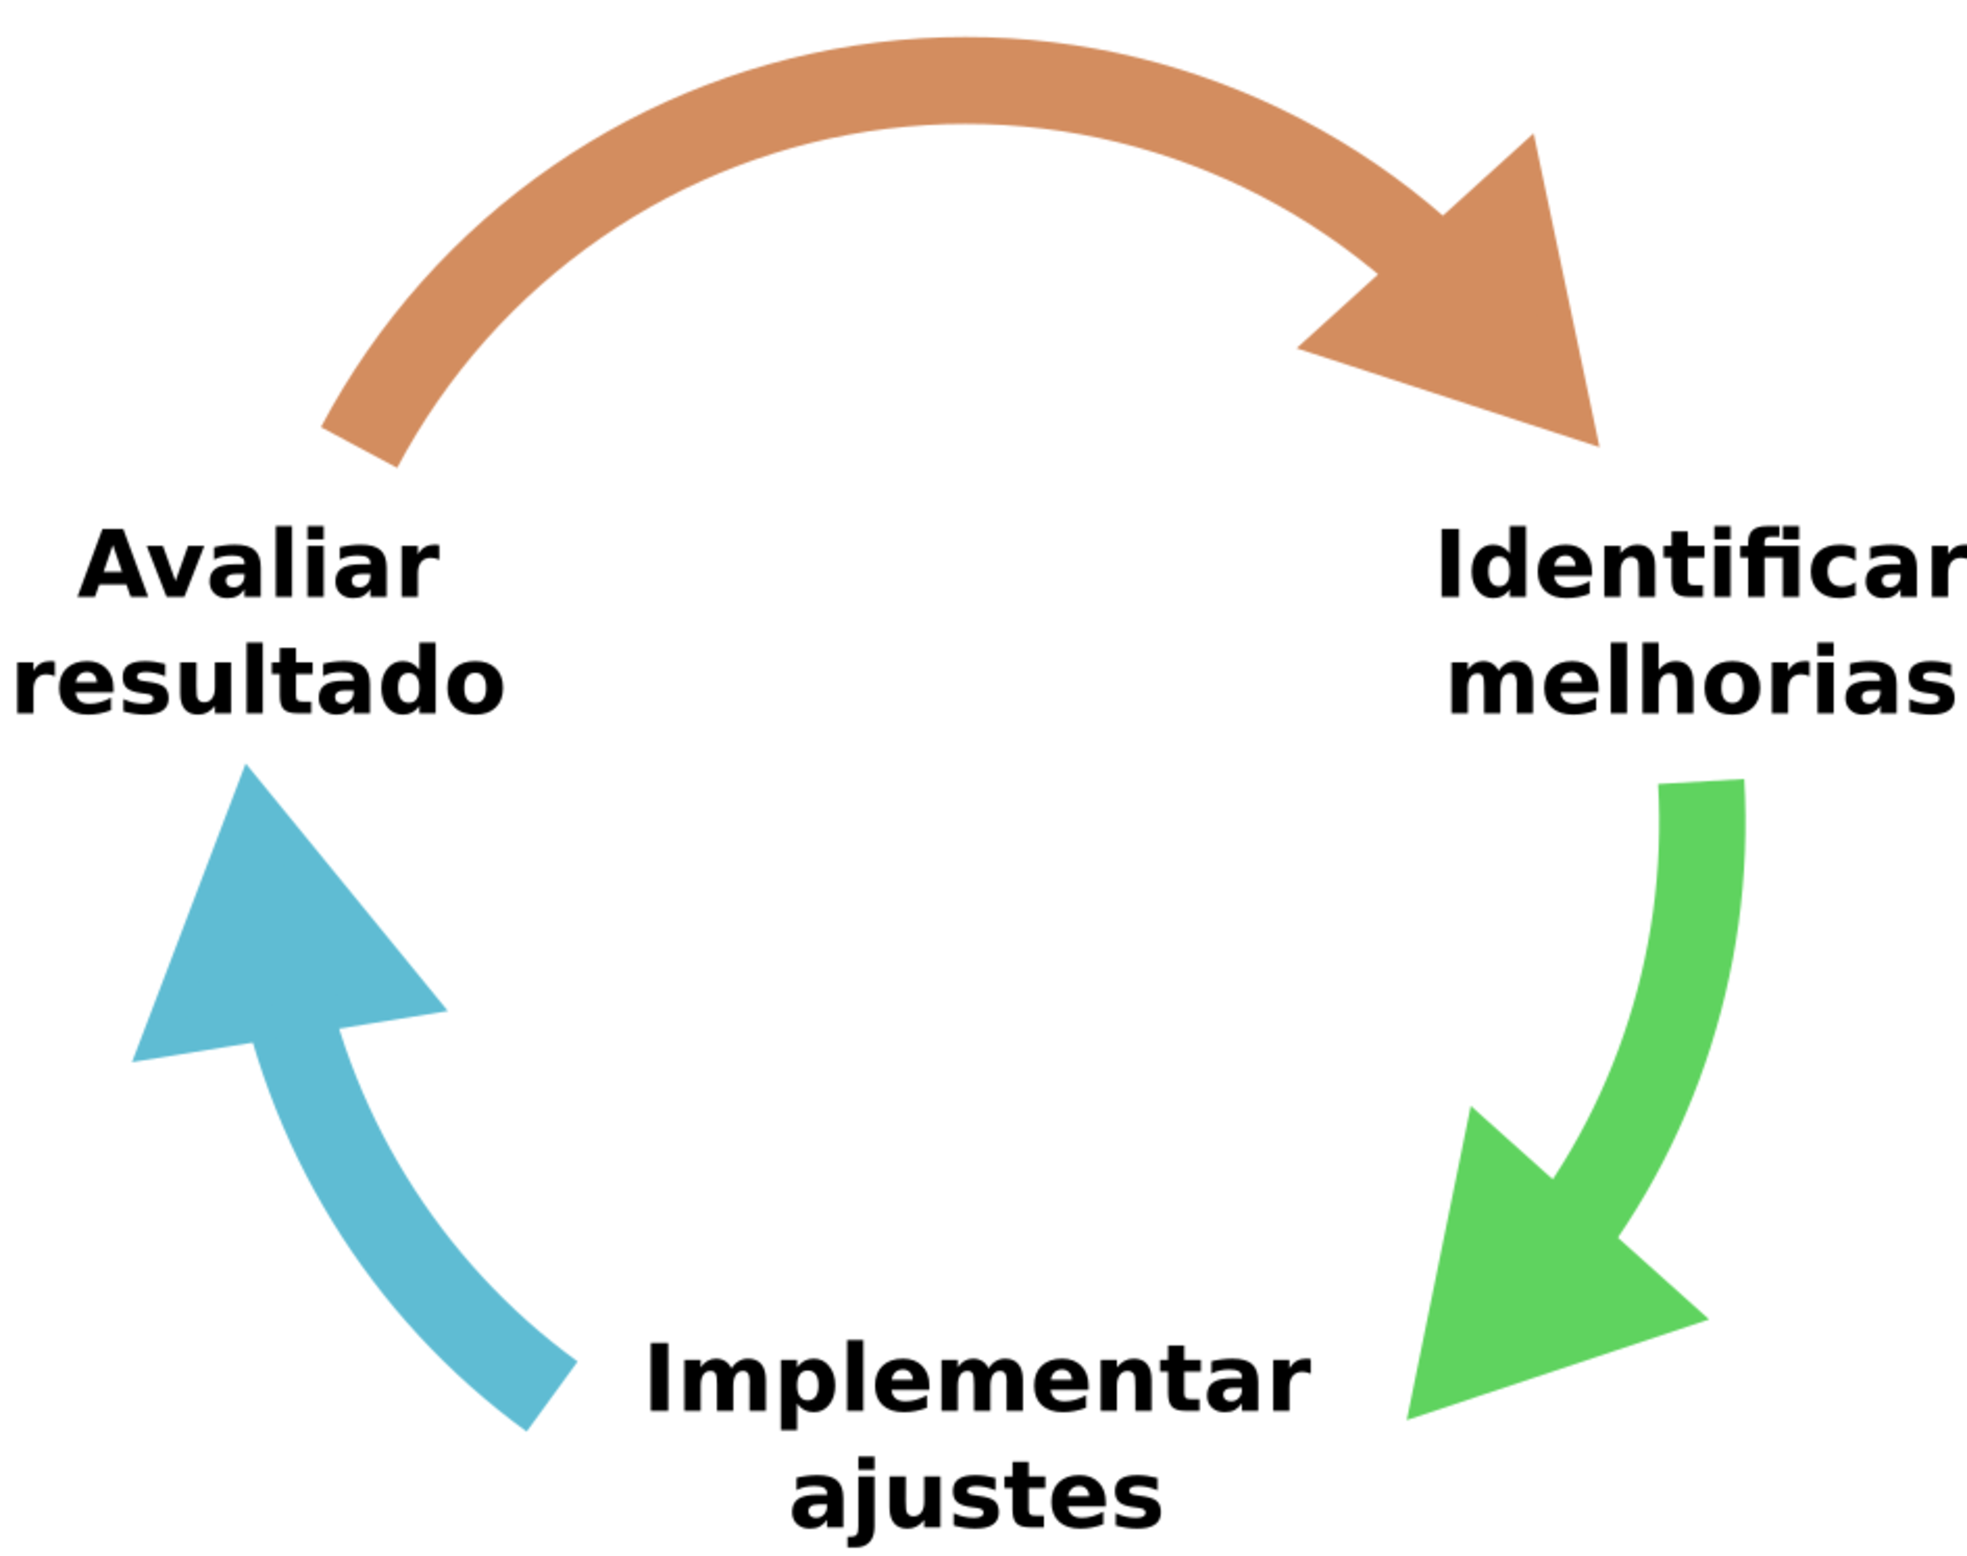
\includegraphics[width=0.4\linewidth]{metodologia}}
        {Fonte: O autor (2025)}
    \label{fig:metodologia}
\end{figure}

\lipsum[39-41]

\chapter{Desenvolvimento do trabalho}\label{cap:desenvolvimento_trabalho}
Essa seção apresenta o que foi realizado no trabalho.

\lipsum[22]

\section{Assunto 1 do desenvolvimento do trabalho}
\lipsum[23-27]

\section{Assunto 2 do desenvolvimento do trabalho}

\lipsum[23-27]

\begin{enumerate}
    \item Exemplo de litstagem enumerada de algoritmo\index{algoritmo};
    \item Outro exemplo de de litstagem enumerada;
    \item Último exemplo de listagem enumerada.
\end{enumerate}

\lipsum[28]:

\begin{itemize}
    \item Exemplo de listagem com bullets;
    \item Outro exemplo de listagem com bullets; 
    \item Exemplo final de listagem com bullets. 
\end{itemize}


\chapter{Experimentos}\label{cap:experimentos}

Nesse capítulo será abordado o escopo dos experimentos, em qual ambiente foram executados, os detalhes dos datasets utilizados bem como a metodologia definida para a sua execução. 

\section{Ambiente utilizado}


\subsection{Configurações de hardware}

Os experimentos foram realizados utilizando a seguinte configuração de hardware\index{hardware}:

\begin{itemize}
    \item Processador\index{processador}: Intel\textsuperscript{\tiny{\copyright}} Core\textsuperscript{\tiny{TM}} i9-13900KF 
    \begin{itemize}
        \item Núcleos: 20
        \item Threads: 32
        \item Velocidade: 5.40GHz
    \end{itemize}
    \item Memória RAM: 64 GB
    \item SSD M2: 1.8 TB
    \item Placa de vídeo: NVIDIA GeForce RTX 4060, 8GB
\end{itemize}

\subsection{Configurações de software}

Os seguintes configurações e componentes de software\index{software} foram utilizados durante a sua execução:

\begin{itemize}
    \item Sistema Operacional: Linux Mint 22, kernel 6.8.0-41-generic
    \item Python (3.12.8) 
    \item Conda (24.11.3) 
    \item Matplotlib (3.9)
\end{itemize}

\section{Exemplo de Section do experimento}

\lipsum[7]

\begin{equation} 
DP = (T_p - T_s) / T_s * 100
\label{eq:diferenca_percentual}
\end{equation}

A equação \eqref{eq:diferenca_percentual} apresentada em a diferença percentual entre o tempo serial e o tempo paralelo de execução. 

\lipsum[1-2]



\subsection{Exemplo de subsection do experimento}

\lipsum[8]
A Tabela \ref{tab:tabelaexemplo1}, apresenta as informações \lipsum[9]

Foram descartadas as observações que possuíam valores nulos, e os atributos que não eram do tipo numérico.
\begin{table}
\caption{Exemplo de tabela de uso genérico}
\begin{center}
\fontsize{10pt}{13pt}\selectfont
\begin{tabular}{lcccc}
\hline
  Base de dados & Observações  &   Features   &   Classe      & Desbalanceamento\\
                & (used/total) & (used/total) & (used/total)  &                 \\
\hline
       Dataset1 &   150/150    &     4/4      &     3/3       & 1.00            \\
       Dataset3 &   208/208    &    60/60     &     2/2       & 1.14            \\
       Dataset3 &   214/214    &     9/10     &     6/7       & 8.44            \\
\hline
\multicolumn{5}{l}{Fonte: O autor (2025)}
\end{tabular}
\label{tab:tabelaexemplo1}
\end{center}
\end{table}


\subsubsection{Exemplo de subsubsection do experimento}

\lipsum[10-12]


\chapter{Resultados}\label{cap:resultados}

Essa seção presenta os resultados do experimento \lipsum[11]

\section{Resultados do experimento}

\lipsum[12-13]

Na Tabela \ref{tab:resultados} foram tabulados todos os dados de resultados das execuções dos experimentos. 

A tabela apresenta uma listagem \lipsum[14]

\lipsum[15-17]

\subsection{Análise dos resultados}
Ao avaliar os dados da Tabela \ref{tab:resultados}, é possível realizar algumas observações de cunho mais geral:

\lipsum[18]


\begin{table}
\caption{Tempos treinamento, predição e acurácia}
\begin{center}
\fontsize{10pt}{13pt}\selectfont
\begin{tabular}{lccc}
\hline
Dataset                       & Tipo processamento  &   Tempo Predict (s)    &Acurácia1 (\%) \\
\hline
\textit{Iris}                 & Serial              &  0.0287 (0.005281)     & 94.24 (1.41)  \\
                              & CPU Multiprocesso   &  0.0272 (0.000206)     & 93.22 (0.91)  \\
                              & GPU                 &  0.0279 (0.000537)     & 93.31 (1.64)  \\
\hline
\textit{Sonar}                & Serial              &  0.0718 (0.000702)     & 85.26 (1.67)  \\
                              & CPU Multiprocesso   &  0.0705 (0.000369)     & 86.36 (1.69)  \\
                              & GPU                 &  0.0703 (0.000834)     & 85.80 (1.18)  \\
\hline
\textit{Glass Identification} & Serial              &  0.0575 (0.000698)     & 67.91 (1.97)  \\
                              & CPU Multiprocesso   &  0.0577 (0.000530)     & 68.40 (1.84)  \\
                              & GPU                 &  0.0571 (0.000587)     & 67.66 (1.76)  \\
\hline
\textit{Libras Movement}      & Serial              &  0.2050 (0.001077)     & 80.06 (1.24)  \\
                              & CPU Multiprocesso   &  0.2020 (0.001227)     & 80.59 (1.16)  \\
                              & GPU                 &  0.2022 (0.001252)     & 80.34 (1.03)  \\
\hline
\multicolumn{4}{l}{Fonte: O autor (2025)}
\end{tabular}
\label{tab:resultados}
\end{center}
\end{table}


A medida de aceleração %informação do speedup pode ser 
foi calculada pela Equação~\eqref{eq:speedup}, onde \(A\) é a \textit{aceleração}, \(T_s\) é o tempo de execução serial/sequencial e \(T_p\) é o tempo de execução paralelo. Dessa forma é possível analisar quantas vezes o desempenho em relação ao tempo sequencial foi impactado pela quantidade de processos utilizados. Quanto maior o número, mais rápido o algoritmo foi executado. 

\begin{equation} 
A = T_s / T_p
\label{eq:speedup}
\end{equation}

\input{2-textos/conclusao}

%Includes pós-textuais
\newpage
%Altera o nome da seção de bibliografia
\renewcommand{\bibname}{\normalsize\centerline{\bfseries\uppercase{Referências}}}

\phantomsection
\addcontentsline{toc}{chapter}{REFERÊNCIAS} % Adiciona a bibliografia ao índice

\printbibliography

\newpage
\phantomsection
\addcontentsline{toc}{chapter}{GLOSSÁRIO} % Adiciona o glossário
\begin{center}
\textbf{\MakeUppercase{Glossário}}
\end{center}

\noindent\textbf{ABNT:} Associação Brasileira de Normas Técnicas, associação civil de utilidade pública responsável pela elaboração das Normas Brasileiras (ABNT NBR).

\vspace{10pt}\noindent\textbf{Acessibilidade:} possibilidade e condição de alcance, percepção e entendimento para utilização, com segurança e autonomia, de espaços, mobiliários, equipamentos urbanos, edificações, transportes, informação e comunicação, inclusive seus sistemas e tecnologias, bem como outros serviços e instalações abertos ao público, de uso público ou privado de uso coletivo, tanto na zona urbana como na rural, por pessoa com deficiência ou mobilidade reduzida.

\vspace{10pt}\noindent\textbf{Beiral:} prolongamento do telhado que excede a prumada de uma parede externa da edificação.

\vspace{10pt}\noindent\textbf{Cisterna:} reservatório subterrâneo ou no nível do solo utilizado para armazenamento de água.

\vspace{10pt}\noindent\textbf{Cota:} medida de distância entre dois pontos, expressa em centímetros.

\vspace{10pt}\noindent\textbf{Cota de nível} medida de distância vertical em relação à Referência de Nível, expressa em metros.

\vspace{10pt}\noindent\textbf{Declividade:} é a razão ou divisão entre a diferença da altura entre dois pontos considerados e a distância horizontal entre esses pontos, expressa em porcentagem.

\vspace{10pt}\noindent\textbf{Duto de ventilação:} espaço vertical ou horizontal delimitado no interior de uma edificação destinado, entre outros fins à ventilação.

\vspace{10pt}\noindent\textbf{Edícula:} edificação secundária e acessória da moradia, geralmente situada no fundo do lote, que não constitui domicílio independente.

\vspace{10pt}\noindent\textbf{Eixo transversal do lote:} eixo que conecta o meio das divisas em linha reta localizado no ponto médio das mesmas.

\vspace{10pt}\noindent\textbf{Fachada:} elevação das partes externas de uma edificação.

\vspace{10pt}\noindent\textbf{Guarda-corpo:} elemento construído de proteção vertical que delimita as faces laterais de escadas, rampas, patamares, terraços, sacadas, mezaninos, passarelas, e galerias.

\vspace{10pt}\noindent\textbf{Guia ou meio-fio:} borda física instalada ao longo das vias, de acabamento da calçada ou passeio, junto à sarjeta (escoamento pluvial), podendo ser rebaixada em casos de acesso de 
veículos e pedestres.

\vspace{10pt}\noindent\textbf{Logradouro público:} área de terra de propriedade pública e de uso comum e/ou especial  do povo destinada às vias de circulação, às praças e aos espaços livres.

\vspace{10pt}\noindent\textbf{Lote:} terreno oriundo de processo regular de parcelamento do solo, com acesso e  testada para logradouro público, servido de infraestrutura básica.

\vspace{10pt}\noindent\textbf{Mansarda:} abertura ou janela que se projeta além da água do telhado de uma  edificação.

\vspace{10pt}\noindent\textbf{Nível do pavimento térreo (NT):} nível atribuído ao piso acabado do pavimento térreo e  determinado pela Referência de Nível (RN) acrescida de no máximo 1,20m (um metro e vinte centímetros).

\vspace{10pt}\noindent\textbf{Passeio:} parte da via de circulação ou logradouro público destinada ao tráfego de pedestres.

\vspace{10pt}\noindent\textbf{Pavimento:} volume compreendido entre lajes de uma edificação.

\vspace{10pt}\noindent\textbf{Pé direito:} distância vertical entre o piso e o teto de um compartimento.

\vspace{10pt}\noindent\textbf{Rampa:} plano inclinado com declividade igual ou superior a 5\% (cinco por cento) de inclinação que interliga dois níveis distintos de piso.

\vspace{10pt}\noindent\textbf{Recuo frontal ou recuo da testada do lote:} é a menor distancia entre uma edificação e a testada do lote onde se situa, medida perpendicularmente em relação à testada do lote, a partir do ponto mais avançado da edificação.

\vspace{10pt}\noindent\textbf{Reservatório de Retardo:} dispositivo aberto ou fechado capaz de reter parte das águas pluviais e liberá-las de forma controlada nas galerias responsáveis de drenagem pública.

\vspace{10pt}\noindent\textbf{Sótão:} espaço utilizável sob a cobertura inclinada, no qual não se admite a elevação de paredes no perímetro da edificação além daquela necessária à estrutura da própria cobertura.

\vspace{10pt}\noindent\textbf{Subsolo:} pavimento situado em nível abaixo da laje do Nível do pavimento térreo (NT).

\vspace{10pt}\noindent\textbf{Talvegue:} linha sinuosa em fundo de vale por onde correm as águas.

\vspace{10pt}\noindent\textbf{Tapume:} vedação provisória do terreno usada durante a construção.

\vspace{10pt}\noindent\textbf{Vistoria:} diligência determinada na forma deste Código para verificar as condições de uma obra, instalação ou exploração de qualquer natureza. % Elemento opcional

\end{document}
